% PCT-SOURCE: pdf=191 print=179 kind=appendix-title id=appendix-recent-developments
% Keep the appendix equation and hyperlink namespace on Appendix A while the
% printed heading remains unlettered, as in the source.
\refstepcounter{section}
\renewcommand{\theHequation}{A.\arabic{equation}}
\section*{APPENDIX}
\phantomsection
\addcontentsline{toc}{section}{Appendix}
\label{sec:appendix-recent-developments}
\begin{center}
  {\Large\bfseries SOME MORE RECENT DEVELOPMENTS IN QUANTUM FIELD THEORY}
\end{center}
\medskip

% PCT-SOURCE: pdf=191 print=179 kind=prose id=appendix-introduction
In the decade and a half since this book was originally written, there has
been important progress in the foundations of quantum field theory. A
systematic review would be out of place here; it would require an addition
whose length would be a substantial fraction of the book. Furthermore, the
interested reader has available the systematic review of Streater \cite{pct-app-1} as well
as the treatise of Bogolubov, Logunov, and Todorov \cite{pct-app-2}, both of which have
extensive bibliographies. The purpose of this Appendix is rather to indicate
three developments which have changed our outlook on the foundations of field
theory as described in the text. These are constructive quantum field theory,
the theory of local algebras, and the theory of superselection rules.

% PCT-SOURCE: pdf=191 print=179 kind=heading id=appendix-constructive-heading
\subsection*{Constructive Quantum Field Theory and the Existence of Non-Trivial Theories of Interacting Fields}
\phantomsection
\addcontentsline{toc}{subsection}{Constructive Quantum Field Theory and the Existence of Non-Trivial Theories of Interacting Fields}
\label{sec:appendix-constructive}

% PCT-SOURCE: pdf=191 print=179 kind=prose id=appendix-constructive-main-problem
In the introduction we described the Main Problem of quantum field theory as:
``either to show that the idealizations involved in the fundamental notions of
the theory (relativistic invariance, quantum mechanics, local fields, etc.) are
incompatible in some physical sense, or to recast the theory in such a form
that it provides a practical language for the description of elementary
particle dynamics.'' It was known in 1964 that the axioms given in Chapter \ref{sec:ch3-fields-and-vacuum-expectation-values}
are consistent because they are satisfied by theories of free fields. On the
other hand, at that time not a single example of a theory of interacting
fields satisfying the axioms was known. Thus a natural first step toward a
solution of the Main Problem was the construction of examples of theories of
interacting fields satisfying the axioms.

% PCT-SOURCE: pdf=191 print=179 kind=prose id=appendix-constructive-origins
Lagrangian quantum field theory offers an abundant supply of models whose
solutions \emph{ought} to satisfy the axioms. Constructive quantum field
theory deals with the mathematical constructions necessary to prove that such
solutions exist. It had its beginnings in the early 1960s and by the middle
1970s had become a well-developed industry.

% PCT-SOURCE: pdf=192 print=180 kind=prose id=appendix-constructive-pioneers
It was preceded by the pioneering studies of Friedrichs \cite{pct-app-3} and Segal \cite{pct-app-4} on
the mathematical foundations of quantum field theory, but the work of these
authors did not treat models with coupled quantized fields. Friedrichs' later
book on perturbation theory \cite{pct-app-5} was an inspiration for the work done on models
in the late 1960s. (The possibilities and some of the difficulties of such a
program were reviewed in \cite{pct-app-6} at the outset of constructive quantum field
theory. The survey \cite{pct-app-7} discusses the general significance of axiomatic and
constructive field theory. Part of the following recapitulates some of the
material in these earlier articles; the reader will find more detail and a
more complete bibliography there.)

% PCT-SOURCE: pdf=192 print=180 kind=prose id=appendix-constructive-first-results
The first results obtained in constructive quantum field theory were proofs of
the existence of solutions for simplified versions of some Lagrangian models
in which cutoffs are introduced. For example, the first model considered was a
cutoff version of the model, $Y_4$, in which a spinor field, $\psi$, and a
scalar field, $\varphi$, interact via a Yukawa interaction given by

% PCT-SOURCE: pdf=192 print=180 kind=equation id=appendix-yukawa-interaction
\[
  H_Y = \lambda \int :\bar\psi(x)\psi(x):\,\varphi(x)\,\dd^3\mathbf{x},
\]

% PCT-SOURCE: pdf=192 print=180 kind=prose id=appendix-total-hamiltonian-intro
the total Hamiltonian being given by

% PCT-SOURCE: pdf=192 print=180 kind=equation id=appendix-total-hamiltonian
\[
  H = H_{0\mathrm F}+H_{0\mathrm B}+H_Y.
\]

% PCT-SOURCE: pdf=192 print=180 kind=prose id=appendix-free-hamiltonians
Here $H_{0\mathrm F}$ and $H_{0\mathrm B}$ are the Hamiltonians for a free
spinor field of mass $M_0$ and for a free boson field of mass $m_0$,
respectively \cite{pct-app-8,pct-app-9}, and $\bar\psi=\psi^\dagger\beta$. A cutoff version
of this model is obtained by expanding the fields in Fourier series in a
cubic box, $V$, of volume $|V|$ and keeping only Fourier components of
frequencies $<K$. The corresponding interaction is

% PCT-SOURCE: pdf=192 print=180 kind=equation id=appendix-cutoff-interaction
\[
  H_{Y;V,\kappa}
  = \lambda\int_V :\bar\psi_\kappa(x)\psi_\kappa(x):\,
      \varphi_\kappa(x)\,\dd^3\mathbf{x}.
\]

% PCT-SOURCE: pdf=192 print=180 kind=prose id=appendix-cutoff-hamiltonian
It is customary to replace $H_{0\mathrm F}$ and $H_{0\mathrm B}$ by
$H_{0\mathrm F,V}$ and $H_{0\mathrm B,V}$, respectively, where the latter are
the Hamiltonians for free particles confined to the box $V$ with periodic
boundary conditions. The cutoff total Hamiltonian

% PCT-SOURCE: pdf=192 print=180 kind=equation id=appendix-cutoff-total
\[
  H_{V,\kappa}=H_{0\mathrm F,V}+H_{0\mathrm B,V}+H_{Y;V,\kappa}
\]

% PCT-SOURCE: pdf=192 print=180 kind=prose id=appendix-cutoff-system
then describes a system of an infinite number of degrees of freedom of which
only a finite subset is coupled through the interaction $H_{Y;V,\kappa}$. For
such a Hamiltonian, the interaction is small compared with the free
Hamiltonian in the sense of T.~Kato, and a standard theorem

% PCT-SOURCE: pdf=193 print=181 kind=prose id=appendix-self-adjointness
asserts that the total Hamiltonian is self-adjoint on the domain of the free
Hamiltonian \cite{pct-app-10}. The self-adjointness $H_{V,\kappa}$ guarantees that

% PCT-SOURCE: pdf=193 print=181 kind=equation id=appendix-cutoff-time-evolution
\[
  U_{V,\kappa}(t)=\exp\!\bigl(\ii tH_{V,\kappa}\bigr)
\]

% PCT-SOURCE: pdf=193 print=181 kind=prose id=appendix-cutoff-unitary-group
defines a continuous unitary one-parameter group. $U_{V,\kappa}(t)$ describes
the time development of states and operators in the cutoff theory. Another
important result of the study of this cutoff model is the existence of vacuum
expectation values of products of field operators:

% PCT-SOURCE: pdf=193 print=181 kind=equation id=appendix-vacuum-expectation-A1
\begin{equation}
  \matrixel{\Omega_{0,V,\kappa}}
    {\displaystyle
      \prod_{j=1}^{n}\psi_\kappa(t_j,\mathbf{x}_j)
      \prod_{k=1}^{n}\bar\psi_\kappa(t_k,\mathbf{x}_k)
      \prod_{\ell=1}^{m}\varphi_\kappa(t_\ell,\mathbf{x}_\ell)}
    {\Omega_{0,V,\kappa}}
  \tag{A.1}\label{eq:appendix-vacuum-expectation-A1}
\end{equation}

% PCT-SOURCE: pdf=193 print=181 kind=prose id=appendix-ground-state-cutoff
Here $\ket{\Omega_{0,V,\kappa}}$ is the ground state of $H_{V,\kappa}$. It is
non-degenerate for sufficiently small $\lambda$. For general $\lambda$ it
cannot be excluded that the ground state has a non-trivial degeneracy. If that
occurs, one can define more than one quantity \eqref{eq:appendix-vacuum-expectation-A1}.

% PCT-SOURCE: pdf=193 print=181 kind=prose id=appendix-yukawa-simplicity
The simplicity of this cutoff version of $Y_4$ arises in part from the fact
that the interaction is only linear in the boson field, $\varphi_\kappa$, while
the free Hamiltonian $H_{0\mathrm B}$ is quadratic. Models of a self-coupled
boson field $\varphi_\kappa$, in which the coupling is of higher degree in
$\varphi_\kappa$ than the free Hamiltonian, were studied in \cite{pct-app-11}. Here the
Hamiltonian is again bounded below but only because one insists that the
interaction

% PCT-SOURCE: pdf=193 print=181 kind=equation id=appendix-polynomial-interaction
\[
  H_{1,V,\kappa}=\lambda\int_V :\mathcal{P}(\varphi_\kappa(x)):\,
    \dd^3\mathbf{x}
\]

% PCT-SOURCE: pdf=193 print=181 kind=prose id=appendix-polynomial-hamiltonian
contain a polynomial $\mathcal{P}$ which is bounded below, and $\lambda\geq0$.
The theory, whose Hamiltonian is

% PCT-SOURCE: pdf=193 print=181 kind=equation id=appendix-polynomial-total
\[
  H_{0\mathrm B}+H_{1,V,\kappa},
\]

% PCT-SOURCE: pdf=193 print=181 kind=prose id=appendix-polynomial-theory
describes an infinite number of oscillators, a finite number of which are
coupled. It may be referred to for brevity as cutoff $\mathcal{P}(\varphi)_4$
theory. For it, one can establish the non-degeneracy of the ground state for
all coupling strengths, $\lambda>0$, and the existence of a set of vacuum
expectation values

% PCT-SOURCE: pdf=193 print=181 kind=equation id=appendix-vacuum-expectation-A2
\begin{equation}
  \matrixel{\Omega_{0,V,\kappa}}
    {\displaystyle\prod_{j=1}^{n}\varphi_\kappa(t_j,\mathbf{x}_j)}
    {\Omega_{0,V,\kappa}}
  \tag{A.2}\label{eq:appendix-vacuum-expectation-A2}
\end{equation}

% PCT-SOURCE: pdf=193 print=181 kind=prose id=appendix-cutoff-generalization
These results for cutoff $Y_4$ and cutoff $\mathcal{P}(\varphi)_4$ theories
were generalized to a wide class of cutoff theories of coupled fermion and
boson fields in \cite{pct-app-12}.

% PCT-SOURCE: pdf=193 print=181 kind=prose id=appendix-cutoff-limits
The results just described leave entirely open the question of the existence
of a limiting theory as $|V|\to\infty$ and $K\to\infty$. However, evidence
from statistical mechanics and from the study of the perturbation series makes
the following two conclusions very plausible.

% PCT-SOURCE: pdf=194 print=182 kind=list id=appendix-cutoff-conclusions
\begin{itemize}
\item[(a)] The limit as $K\to\infty$ can only exist in general if extra terms,
  which become infinite as $K\to\infty$, are added to the Hamiltonian. The
  addition of these terms can often be interpreted in terms of a
  renormalization of the basic parameters of the theory.
\item[(b)] Not all quantities associated with the theory may be expected to
  have well-defined limits as $|V|\to\infty$ and $K\to\infty$. However, the
  vacuum expectation values \eqref{eq:appendix-vacuum-expectation-A1} and \eqref{eq:appendix-vacuum-expectation-A2} are reasonable candidates for
  convergence, since each term of the perturbation series for them is known to
  converge as $|V|\to\infty$ and $K\to\infty$, once the renormalizations
  mentioned under (a) have been carried out.
\end{itemize}

% PCT-SOURCE: pdf=194 print=182 kind=prose id=appendix-renormalization-step
The second logical step toward the construction of solutions was then to prove
that such limits exist. However, what actually happened was more complicated.
The process of renormalization was first controlled in an even simpler model,
in which the $|V|\to\infty$ limit posed no problem at all. This was a theory of
non-relativistic fermions coupled to relativistic mesons. Here the Hamiltonian
is

% PCT-SOURCE: pdf=194 print=182 kind=equation id=appendix-nonrelativistic-hamiltonian
\[
  H_\kappa=(2M)^{-1}\int
    \boldsymbol{\nabla}\psi^\dagger(\mathbf{x})\!\cdot\!
    \boldsymbol{\nabla}\psi(\mathbf{x})\,\dd^3\mathbf{x}
    +H_{0\mathrm B}
    +g\int\psi^\dagger(\mathbf{x})\psi(\mathbf{x})
      \varphi_\kappa(\mathbf{x})\,\dd^3\mathbf{x}.
\]

% PCT-SOURCE: pdf=194 print=182 kind=prose id=appendix-nucleon-number
The fermion field $\psi$ describes non-relativistic nucleons whose number

% PCT-SOURCE: pdf=194 print=182 kind=equation id=appendix-number-operator
\[
  N=\int\psi^\dagger(\mathbf{x})\psi(\mathbf{x})\,\dd^3\mathbf{x}
\]

% PCT-SOURCE: pdf=194 print=182 kind=prose id=appendix-number-conservation
is exactly conserved

% PCT-SOURCE: pdf=194 print=182 kind=equation id=appendix-number-commutator
\[
  [H_\kappa,N]=0.
\]

% PCT-SOURCE: pdf=194 print=182 kind=prose id=appendix-renormalized-hamiltonian
The renormalization process corresponds to the replacement of $H_\kappa$ by
$H_\infty=\lim_{\kappa\to\infty}(H_\kappa-N\,\Delta E_\kappa)$,
% PCT-SOURCE: pdf=194 print=182 kind=prose id=appendix-self-energy
where $\Delta E_\kappa$ is the lowest-order self-energy of a nucleon arising
from the meson--nucleon interaction. It was shown that
$\exp\!\bigl[\ii t(H_\kappa-N\,\Delta E_\kappa)\bigr]$

% PCT-SOURCE: pdf=194 print=182 kind=prose id=appendix-renormalized-group
converges to the continuous unitary one-parameter group
$\exp(\ii tH_\infty)$ \cite{pct-app-13}. (This is more than one expects for general models.)
Furthermore, the vacuum expectation values \eqref{eq:appendix-vacuum-expectation-A1} converge \cite{pct-app-14}.

% PCT-SOURCE: pdf=194 print=182 kind=prose id=appendix-vacuum-polarization
The preceding results on the non-relativistic model represented a fundamental
step forward because they give a non-perturbative treatment of a non-trivial
renormalization. However, they did not involve the full complications of a
relativistic theory because the model does not predict a non-trivial vacuum
polarization. The next stage in the development of the theory had to deal with
the phenomenon of vacuum polarization and required essentially new ideas. The
technical difficulties were so great that several workers had the genial idea
to consider the models first in space-times of lower dimension, where the

% PCT-SOURCE: pdf=195 print=183 kind=prose id=appendix-lower-dimension
singularities of the fundamental solutions of the wave equation are less
violent \cite{pct-app-15,pct-app-16,pct-app-17,pct-app-18,pct-app-19}.

% PCT-SOURCE: pdf=195 print=183 kind=prose id=appendix-phi4-two-dimensional
The $\lambda(\varphi^4)_2$ model has, if one believes the evidence of its
solution by perturbation series in $\lambda$, no ultraviolet divergences, but
does have non-trivial vacuum polarization. Thus, it is a suitable test case
for existence theorems. The Hamiltonian of the $\lambda(\varphi^4)_2$ model in
a box is a well-defined hermitian operator when the $\varphi^4$ is understood
as Wick-ordered. However, the Hamiltonian is not obviously bounded below,
since the Wick-ordering destroys the formal positivity of $\varphi^4$.

% PCT-SOURCE: pdf=195 print=183 kind=prose id=appendix-phi4-probabilistic
This problem was solved in a paper \cite{pct-app-15} which contained a number of
mathematical ideas which were important for later developments. In particular,
it first used the probabilistic methods later associated with Euclidean field
theory to study the semi-group
$\bigl\{\exp[-tH_{\kappa,V}];\,0\leq t<\infty\bigr\}$.

% PCT-SOURCE: pdf=195 print=183 kind=prose id=appendix-multiplication-operator
In the realization of $H_V$ thereby obtained,
$H_{1,V}=\lambda\int_V :\varphi^4:\,\dd x$

% PCT-SOURCE: pdf=195 print=183 kind=prose id=appendix-multiplication-description
is a multiplication operator on a space of square-integrable functions. It is
not bounded below, but the sets on which it is large and negative are so small
in measure that the addition of the positive $H_0$ makes the sum
$H_V=H_0+H_{1,V}$

% PCT-SOURCE: pdf=195 print=183 kind=prose id=appendix-positive-sum-conclusion
bounded below.

% PCT-SOURCE: pdf=195 print=183 kind=prose id=appendix-yukawa-two-dimensional
The next most difficult case after the $\lambda(\varphi^4)_2$ model is $Y_2$,
the theory of a scalar or pseudo-scalar boson field coupled to a fermion field.
It requires an infinite boson mass renormalization and an infinite vacuum
energy renormalization. The Hamiltonian of $Y_2$ was constructed and proved
bounded below in \cite{pct-app-16,pct-app-17,pct-app-19}.

% PCT-SOURCE: pdf=195 print=183 kind=prose id=appendix-phi4-three-dimensional
For $\lambda(\varphi^4)_3$, the $\varphi^4$ theory in three-dimensional
space-time, the situation is even more complicated. The ultraviolet
divergences are sufficiently bad that the Fock representation of the
commutation relations cannot be used to make the Hamiltonian in a box well
defined: a unitarily inequivalent representation has to be used, constructed
by a process referred to as \emph{wave function renormalization} \cite{pct-app-20}. (For a
discussion of a class of models which puts wave function renormalization in a
more general context, see \cite{pct-app-21}.) The proof that the renormalized
$\lambda(\varphi^4)_3$ Hamiltonian is bounded below remained an open problem
for several years until finally, by an extraordinary effort, it was solved in
\cite{pct-app-22}.

% PCT-SOURCE: pdf=195 print=183 kind=prose id=appendix-box-results
The work quoted in \cite{pct-app-15,pct-app-16,pct-app-17,pct-app-18,pct-app-19,pct-app-20,pct-app-21,pct-app-22} shows that a renormalized Hamiltonian in a box but
free of ultraviolet cutoffs and bounded below can be constructed for the
$\lambda(\varphi^4)_2$, $Y_2$, and $\lambda(\varphi^4)_3$ models. The next
problem was to get rid of the box. Here the decisive ideas were these [23, 18,
24]:

% PCT-SOURCE: pdf=195 print=183 kind=list id=appendix-local-hamiltonian-strategy
\begin{itemize}
\item[(c)] Because of Haag's theorem, one cannot expect an interaction term
  such as $\lambda\int :\varphi^4:\,\dd x$ integrated over all space to make
  sense, even

% PCT-SOURCE: pdf=196 print=184 kind=prose id=appendix-local-hamiltonian-continuation
for the least singular case of two dimensions. However, one does expect

% PCT-SOURCE: pdf=196 print=184 kind=equation id=appendix-local-hamiltonian
\[
  H_1(g)=\lambda\int \dd x\,g(x):\varphi^4:(x)
\]

% PCT-SOURCE: pdf=196 print=184 kind=prose id=appendix-local-hamiltonian-cutoff
to make sense if $g(x)$ is a smooth positive function vanishing outside some
bounded region. If $g(x)=1$ in some region, then

% PCT-SOURCE: pdf=196 print=184 kind=equation id=appendix-local-hamiltonian-total
\[
  H(g)=H_0+H_1(g)
\]

% PCT-SOURCE: pdf=196 print=184 kind=prose id=appendix-local-hamiltonian-domain
ought to serve as a correct \emph{local Hamiltonian} in the dependence domain
of the region where $g=1$ (see Figure~\ref{fig:A-1}). That means that

% PCT-SOURCE: pdf=196 print=184 kind=equation id=appendix-local-time-development
\[
  \varphi(t,\mathbf{x})
  =\exp\!\bigl(\ii H(g)t\bigr)\varphi(0,\mathbf{x})
    \exp\!\bigl(-\ii tH(g)\bigr)
\]

% PCT-SOURCE: pdf=196 print=184 kind=prose id=appendix-local-time-development-text
should be independent of $g$ and give the correct time dependence of the field
$\varphi$ as long as $\{t,\mathbf{x}\}$ stays in the diamond indicated in
Figure~\ref{fig:A-1}.

% PCT-SOURCE: pdf=196 print=184 kind=figure id=fig:appendix-dependence-domain
\begingroup
\renewcommand{\thefigure}{A.1}
\renewcommand{\figurename}{Figure}
\begin{figure}[htbp]
  \centering
  \begin{tikzpicture}[>=Stealth,line cap=round,line join=round]
    % The causal diamond and its horizontal diagonal.
    \draw[line width=.85pt]
      (-3.15,0) -- (0,3.15) -- (3.15,0) -- (0,-3.15) -- cycle;
    \draw[line width=.85pt] (-3.15,0) -- (3.15,0);

    % The space and time axes, both set off from the diamond as in the source.
    \draw[->,line width=.7pt] (3.67,0) -- (5.67,0) node[right=2pt] {$x$};
    \draw[->,line width=.7pt] (3.15,1.20) -- (3.15,2.66);
    \node[anchor=west] at (3.30,1.90) {$t$};

    % The interval on which g=1.
    \draw[line width=.55pt] (-3.15,-0.14) -- (-3.15,-1.10);
    \draw[line width=.55pt] ( 3.15,-0.14) -- ( 3.15,-1.10);
    \draw[<->,line width=.6pt] (-3.09,-0.76) -- (3.09,-0.76);
    \node[fill=white,inner sep=1.5pt] at (0,-0.76) {$g=1$};
  \end{tikzpicture}
  \caption{The dependence domain of the region where $g=1$.}
  \label{fig:A-1}
\end{figure}
\endgroup


% PCT-SOURCE: pdf=196 print=184 kind=list-continuation id=appendix-local-algebras
\item[(d)] Although $H(g)$ does not converge as $g\to1$, the family of such
  $H(g)$ defines a unique automorphism of local algebras. That means that if
  $F$ is a bounded function of the smeared fields

% PCT-SOURCE: pdf=196 print=184 kind=equation id=appendix-smeared-field
\[
  \varphi(f)=\int\dd t\,\dd x\,f(t,x)\varphi(t,x)
\]

% PCT-SOURCE: pdf=196 print=184 kind=prose id=appendix-smeared-field-support
with $f$ having support in some bounded region, $\mathcal{O}$, then

% PCT-SOURCE: pdf=196 print=184 kind=equation id=appendix-local-automorphism
\[
  \alpha_\tau F(\varphi(f))=F(\varphi(f_\tau)),
  \qquad f_\tau(\tau,x)\equiv f(t,x)
\]

% PCT-SOURCE: pdf=196 print=184 kind=prose id=appendix-local-automorphism-text
is independent of $g$ as soon as the region where $g$ is $1$ gets sufficiently
large in both directions. The result is then to be interpreted: one has

% PCT-SOURCE: pdf=197 print=185 kind=prose id=appendix-right-local-algebras
the right local algebras and the right automorphism of them but the
representation is the wrong representation because the automorphism
$\alpha_\tau$ is not an inner automorphism; i.e., there is no unitary operator
$V(\tau)$ such that

% PCT-SOURCE: pdf=197 print=185 kind=equation id=appendix-inner-automorphism
\[
  \alpha_\tau(A)=V(\tau)A V(\tau)^\dagger.
\]

% PCT-SOURCE: pdf=197 print=185 kind=prose id=appendix-no-global-hamiltonian
This implies, in particular, that there is no self-adjoint operator $H$ such
that

% PCT-SOURCE: pdf=197 print=185 kind=equation id=appendix-inner-time-evolution
\[
  \alpha_\tau(A)=\exp(\ii H\tau)A\exp(-\ii H\tau).
\]

% PCT-SOURCE: pdf=197 print=185 kind=list-continuation id=appendix-gns
\item[(e)] To get the right representation one must construct a vacuum
  functional on the local algebras, and then appeal to the
  Gelfand--Naimark--Segal (GNS) theorem. This asserts that, to every
  functional, $\rho$, there is a vector $\ket{\Psi_\rho}$ in some Hilbert
  space $\mathcal{H}_\rho$, such that $\rho$ is given by the expectation value
  in the state $\ket{\Psi_\rho}$. The theorem, which is stated precisely on
  p.~192, actually constructs $\mathcal{H}_\rho$ and the representation of the
  algebra in question, in a manner similar to the ``Reconstruction Theorem''
  of Section 3.4; see \cite{pct-app-67}. The idea is to use the local Hamiltonians to
  construct approximate vacuum states. The state,
  $\ket{\Omega_{0,V}}$, is now chosen as the ground state,
  $\ket{\Omega_0(g)}$, of the $H(g)$; it is proved non-degenerate. One regards
  $\matrixel{\Omega_0(g)}{A}{\Omega_0(g)}=\rho_g(A)$ as a linear functional on
  the local algebras and looks for convergent sequences $\rho_{g_i}$. The
  limiting states and their associated representations are candidates for the
  correct physical representation in which the axioms are satisfied.
\end{itemize}

% PCT-SOURCE: pdf=197 print=185 kind=prose id=appendix-hamiltonian-strategy
The extraordinary theoretical structure which was erected to fulfil these
ideas is reviewed in \cite{pct-app-25} and \cite{pct-app-26}. It is sometimes referred to as the
\emph{Hamiltonian strategy} in constructive quantum field theory. The results
obtained for $(\varphi^4)_2$, the $\varphi^4$ theory in two-dimensional
space-time, were soon extended to $\mathcal{P}(\varphi)_2$ where $\mathcal{P}$
is any polynomial bounded below \cite{pct-app-18,pct-app-27}.

% PCT-SOURCE: pdf=197 print=185 kind=prose id=appendix-euclidean-strategy-start
We have already noted that in the work just quoted, it was found useful to
study a Hamiltonian such as $H(g)$ via the associated semi-group
$\bigl\{\exp[-tH(g)];\,0\leq t<\infty\bigr\}$.

% PCT-SOURCE: pdf=197 print=185 kind=prose id=appendix-euclidean-strategy
In the context of a relativistic theory this can be regarded as a Euclidean
method since the substitution $t\to\ii t$ converts the Minkowski metric
$-c^2t^2+\mathbf{x}^2$ into a Euclidean metric. Now, parallel to the
Hamiltonian strategy, there had developed in the 1960s the \emph{Euclidean
strategy} in which one works with imaginary time vacuum expectation values
(or Green's functions). The idea, fundamental for the Euclidean strategy,
that the analytic continuation of the Green functions to imaginary times
should define the correlation functions of a Euclidean field theory goes back
to Schwinger and Nakano \cite{pct-app-28,pct-app-29}. It was extensively explored by Symanzik
\cite{pct-app-30,pct-app-31,pct-app-32}.

% PCT-SOURCE: pdf=198 print=186 kind=prose id=appendix-euclidean-formalism
The beauty of the Euclidean formalism is that it promises to give
mathematical meaning to the celebrated solution of quantum field theory by
quadratures. The formula in question is, for the case of a single self-coupled
Bose field,

% PCT-SOURCE: pdf=198 print=186 kind=equation id=appendix-euclidean-gell-mann-low
\[
  \ev{\varphi(x_1)\cdots\varphi(x_k)}
  =Z^{-1}\int\prod_{j=1}^{k}\varphi_E(x_j)\,
    \dd\mu_{m_0^2}(\varphi_E)\,
    \exp\!\left[\int\mathcal{L}_I(\varphi_E(x))\,\dd^n x\right]
\]

% PCT-SOURCE: pdf=198 print=186 kind=prose id=appendix-gell-mann-low-text
(commonly known as the Euclidean Gell--Mann--Low formula). Here $n$ is the
space-time dimension

% PCT-SOURCE: pdf=198 print=186 kind=equation id=appendix-partition-function
\[
  Z=\int\dd\mu_{m_0^2}(\varphi_E)\,
    \exp\!\left[\int\mathcal{L}_I(\varphi_E(x))\,\dd^n x\right]
\]

% PCT-SOURCE: pdf=198 print=186 kind=prose id=appendix-gaussian-measure
and $\dd\mu_{m_0^2}(\varphi_E)$ is the Gaussian probability measure of mean
zero and covariance

% PCT-SOURCE: pdf=198 print=186 kind=equation id=appendix-gaussian-covariance
\[
  \int\varphi_E(x)\varphi_E(y)\,\dd\mu_{m_0^2}(\varphi_E)
  =\bigl[(-\Delta+m_0^2)^{-1}\bigr](x,y).
\]

% PCT-SOURCE: pdf=198 print=186 kind=prose id=appendix-euclidean-interaction
(For an introduction to the required notions of probability theory see \cite{pct-app-33}.)
$\mathcal{L}_I(\varphi_E)$ is the interaction Lagrangian density of the
theory; for the $\lambda\mathcal{P}(\varphi)_2$ theory, for example, it is
$-\lambda\mathcal{P}(\varphi_E(x))$.

% PCT-SOURCE: pdf=198 print=186 kind=prose id=appendix-euclidean-cutoffs
The formula for the Schwinger functions does not make sense as it stands, but
if an ultraviolet and a box cutoff are introduced, it is perfectly well
defined and can serve as a starting point for the construction of the theory
free of cutoffs.

% PCT-SOURCE: pdf=198 print=186 kind=prose id=appendix-reconstruction-missing
What was lacking in Euclidean field theory, even at the end of the 1960s, was a
reconstruction theorem which would permit one to pass from the solution of a
Euclidean field theory to a corresponding quantum field theory in Minkowski
space, satisfying assumptions 0, I, II, and III of Chapter \ref{sec:ch3-fields-and-vacuum-expectation-values} (pp.~96--102).

% PCT-SOURCE: pdf=198 print=186 kind=prose id=appendix-reconstruction-theorem
Such a reconstruction theorem was provided in \cite{pct-app-34}, where it was shown that
there is a natural extension to Euclidean field theory of the Markov property
usually defined for stochastic processes, and that it, together with a few
other properties, suffices for the return via analytic continuation from the
Euclidean correlation functions (Schwinger functions) to a set of vacuum
expectation values for a theory satisfying 0, I, II, and III.

% PCT-SOURCE: pdf=198 print=186 kind=prose id=appendix-euclidean-encouragement
Two other papers also seem to have provided a considerable encouragement to
people to think Euclidean. In \cite{pct-app-35} it was shown that

% PCT-SOURCE: pdf=199 print=187 kind=prose id=appendix-nelson-symmetry-intro
the existence of a vacuum energy per unit volume in $\mathcal{P}(\varphi)_2$
theories follows from the striking symmetry (Nelson symmetry)

% PCT-SOURCE: pdf=199 print=187 kind=equation id=appendix-nelson-symmetry
\[
  \matrixel{\Omega_0}{\exp(-tH_1)}{\Omega_0}
  =\matrixel{\Omega_0}{\exp(-tH_t)}{\Omega_0}
\]

% PCT-SOURCE: pdf=199 print=187 kind=prose id=appendix-nelson-hamiltonian-intro
where

% PCT-SOURCE: pdf=199 print=187 kind=equation id=appendix-nelson-hamiltonian
\[
  H_1=H_0+\int_{-1/2}^{1/2}\dd x\,:\mathcal{P}(\varphi(x)):.
\]

% PCT-SOURCE: pdf=199 print=187 kind=prose id=appendix-nelson-ground-state
and $\ket{\Omega_0}$ is the ground state of $H_0$. This identity is an
immediate consequence of the fact that both expressions in question can be
written as functional integrals in which the dependence on the integration
variable, $\varphi_E$, appears in the form of a Euclidean invariant integral
of the function

% PCT-SOURCE: pdf=199 print=187 kind=equation id=appendix-nelson-integral
\[
  \exp\!\left[-\int_{-t/2}^{t/2}\int_{-1/2}^{1/2}
    \dd^2x\,:\mathcal{P}(\varphi_E(x)):\right].
\]

% PCT-SOURCE: pdf=199 print=187 kind=prose id=appendix-nelson-consequence
This is a striking example of an identity which becomes obvious when it is
expressed in appropriate Euclidean language. The second paper was \cite{pct-app-36}, which
gave conditions on Schwinger functions guaranteeing that they should give rise
to a quantum field theory in Minkowski space. Since these conditions are
eminently practical, they gave a strong incentive to the study of Euclidean
field theory models.

% PCT-SOURCE: pdf=199 print=187 kind=prose id=appendix-statistical-mechanics
In Euclidean field theory the relation between statistical mechanics and field
theory is more than an analogy. For boson fields the Schwinger functions are
correlation functions of a certain (somewhat peculiar!) statistical mechanics.
This suggests that the methods by which the thermodynamic limit is controlled
in statistical mechanics should be adaptable to Euclidean field theory.

% PCT-SOURCE: pdf=199 print=187 kind=prose id=appendix-lattice-approximation
A striking application of these ideas is obtained if one approximates the
Euclidean $\varphi^4$ theory by a lattice theory in which Euclidean space is
replaced by a lattice of points. The free Hamiltonian then is chosen as (the
discrete analogue of) the Laplacian with Dirichlet boundary conditions, which
turns out to be effectively a ferromagnet. For $\mathcal{P}$ an even
polynomial plus a linear term, it can then be shown that the Schwinger
functions converge monotonically as the lattice is increased in size,
independently of the lattice spacing \cite{pct-app-37,pct-app-38}.

% PCT-SOURCE: pdf=199 print=187 kind=prose id=appendix-magnetic-field
Another result which is plausible in view of the analogy with the statistical
mechanics of ferromagnets is that of \cite{pct-app-39} in which it is shown that for an
interaction $\lambda\mathcal{P}(\varphi)+\mu\varphi^k$ with
$k<\deg\mathcal{P}$, where $k$ is odd there is a unique vacuum and mass gap
for all sufficiently large $|\mu|$. This is analogous to the behavior of a
ferromagnet: when a ferromagnet is put in a magnetic field, its magnetization
and hence its state is uniquely determined.

% PCT-SOURCE: pdf=200 print=188 kind=prose id=appendix-ising-comparison
For some of the closer comparisons between ferromagnets and
$\mathcal{P}(\varphi)_2$ models and, in particular, for the relation to the
Ising model, it is necessary to restrict the polynomial to one of fourth
degree, which without loss of generality can be taken as

% PCT-SOURCE: pdf=200 print=188 kind=equation id=appendix-fourth-degree-polynomial
\[
  \mathcal{P}(\varphi)=\lambda\varphi^4+\mu\varphi^2+\nu\varphi.
\]

% PCT-SOURCE: pdf=200 print=188 kind=prose id=appendix-unique-vacuum
In \cite{pct-app-40,pct-app-41} it is shown that there is a unique vacuum for $\nu\neq0$.

% PCT-SOURCE: pdf=200 print=188 kind=prose id=appendix-two-solutions
One of the most beautiful results along this line is the proof that for
$\nu=0$ and all sufficiently large negative $\mu$ the
$\mathcal{P}(\varphi)=\lambda\varphi^4+\mu\varphi^2$ theory has at least two
distinct solutions, one in which the expectation value of $\varphi$ in the
ground state, $\ev{\varphi(x)}$, is $>0$ and another for which it is $<0$
\cite{pct-app-42}. Combined with the preceding result, this suggests that the phase diagram
of the $\mathcal{P}(\varphi)=\lambda\varphi^4+\mu\varphi^2+\nu\varphi$
theory in the $\lambda$--$\mu$ plane is similar to that of the Ising model
ferromagnet in the $\beta$--$B$ plane where $\beta=(kT)^{-1}$, $k$ being
Boltzmann's constant, $T$ the absolute temperature, and $B$ the external
magnetic field.

% PCT-SOURCE: pdf=200 print=188 kind=figure id=fig:appendix-ising-phase
% PCT-SOURCE: pdf=200 print=188 kind=figure id=A.2
% Native reconstruction of the Ising phase diagram on source page 188.
\begingroup
\renewcommand{\thefigure}{A.2}
\renewcommand{\figurename}{Figure}
\begin{figure}[htbp]
  \centering
  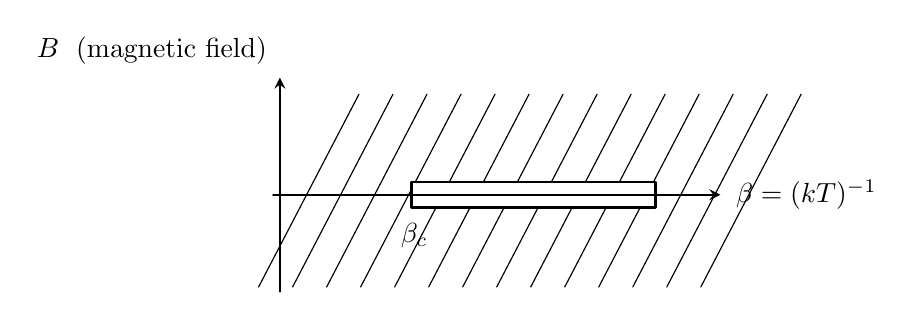
\begin{tikzpicture}[x=1.08cm,y=.96cm,>=stealth,line cap=round,
    line join=round]
    % Diagonal hatching marks the two-phase line's surrounding phase
    % diagram.  The white strip is the B=0 part for beta >= beta_c.
    \foreach \x in {-.25,.15,.55,.95,1.35,1.75,2.15,2.55,2.95,3.35,3.75,4.15,4.55,4.95}
      \draw[line width=.42pt] (\x,-1.22) -- ++(1.18,2.55);

    \draw[->,line width=.75pt] (0,-1.28) -- (0,1.55)
      node[above left=1pt] {$B$\; (magnetic field)};
    \draw[->,line width=.75pt] (-.08,0) -- (5.18,0)
      node[right=2pt] {$\beta=(kT)^{-1}$};

    % The critical half-line lies on B=0.  Its outlined strip preserves the
    % double ruled line visible in the scan.
    \fill[white] (1.55,-.17) rectangle (4.42,.17);
    \draw[line width=.9pt] (1.55,-.17) rectangle (4.42,.17);
    \draw[line width=.55pt] (1.55,0) -- (4.42,0);
    \node[below=2pt] at (1.58,-.17) {$\beta_c$};
  \end{tikzpicture}
  \caption{Phase diagram of the Ising ferromagnet (nearest-neighbor interaction). The phase is unique and the correlation functions decay exponentially for all values of $\beta$ and $B$ except those satisfying $B=0$, $\beta_c\leq\beta<\infty$, where there are exactly two phases. The phase diagram for the $\lambda\varphi^4+\mu\varphi^2+\nu\varphi$ model is similar, with $B$ replaced by $\nu$ and $\beta$ by $\lambda$. The solution is known to be unique for $\nu\ne0$ and for all sufficiently small positive $\lambda$. It is known that at least two solutions, I and II, exist for all sufficiently large $\lambda$ with $\varphi\to-\varphi$ symmetry broken in the sense that $\matrixel{\Omega_{0I}}{\varphi_1(x)}{\Omega_{0I}}=-\matrixel{\Omega_{0II}}{\varphi_1(x)}{\Omega_{0II}}\ne0$.}
  \label{fig:A-2}
\end{figure}
\endgroup


% PCT-SOURCE: pdf=200 print=188 kind=prose id=appendix-return-main-problem
It is time to cease celebrating the successes of Euclidean field theory in
relating the ideas of statistical mechanics to quantum field theory and return
to the Main Problem. The books \cite{pct-app-43} and \cite{pct-app-44} give a more complete survey, with
references complete up to their dates of publication.

% PCT-SOURCE: pdf=200 print=188 kind=prose id=appendix-axiomatic-verification
From the point of view of axiomatic quantum field theory, one of the most
important results achieved (by a combination of the Hamiltonian and Euclidean
strategies) was the verification for the $\lambda\mathcal{P}(\varphi)_2$ model
of assumptions 0, I, II, III of Chapter \ref{sec:ch3-fields-and-vacuum-expectation-values}, i.e., the proof that the
$\lambda\mathcal{P}(\varphi)_2$ model defines (on two-dimensional space-time)
a local relativistic quantum field theory with a cyclic vacuum state. This was
established in \cite{pct-app-45} for any $\mathcal{P}$ bounded below and all sufficiently
small $\lambda$. For $\mathcal{P}$ even plus a linear term but for all
$\lambda$, it was established in \cite{pct-app-37,pct-app-38,pct-app-44}. An

% PCT-SOURCE: pdf=201 print=189 kind=prose id=appendix-axiomatic-alternative
alternative treatment of this case, based on a very neat and powerful
formalism expressing the physical content of the theory in terms of a
generating functional for the Schwinger functions, was given in \cite{pct-app-46,pct-app-47}. This
justified the faith of those who had, for so many years, believed in the
existence of non-trivial local relativistic quantum field theories.

% PCT-SOURCE: pdf=201 print=189 kind=prose id=appendix-skeptical-questions-intro
Of course, the skeptics could still have questions:

% PCT-SOURCE: pdf=201 print=189 kind=questions id=appendix-skeptical-questions
Could the constructed solution be, in fact, trivial?

Does the constructed solution have anything to do with the perturbation series
for the vacuum expectation values traditionally associated with the
$\mathcal{P}(\varphi)_2$ model?

Could asymptotic completeness (assumption IV, p.~102) fail for the model?

Might the existence of a solution be a freak of two dimensions or of the
regularity of the interaction; could the analogous problems for higher
dimensions or for more singular interactions be without non-trivial
solutions?

% PCT-SOURCE: pdf=201 print=189 kind=prose id=appendix-mass-spectrum
An important step toward answering these questions was already taken at the
same time that axioms 0, I, II, and III were verified for small positive
$\lambda$ \cite{pct-app-45}. It was shown that the mass spectrum of the theory has the form
generally expected: Above the unique vacuum state there is a gap, then the
single-particle states of mass $m$, and then another gap. Further, the field has
non-vanishing matrix elements,
$\matrixel{\Omega_0}{\varphi(x)}{\Omega_1}$, between the vacuum,
$\ket{\Omega_0}$, and one-particle states,
$\ket{\Omega_1}$. This information provides the necessary input for the
Haag--Ruelle theory of scattering \cite{pct-app-48,pct-app-49}. The Haag--Ruelle theory constructs
collision states corresponding to ingoing and outgoing beams with arbitrary
numbers of the particles of mass $m$ whose single-particle states occurred in
the hypotheses. The scattering amplitudes are given in terms of the Fourier
transforms of Green's functions evaluated on the mass shell.

% PCT-SOURCE: pdf=201 print=189 kind=prose id=appendix-feynman-rules
It was shown in \cite{pct-app-50} that when smeared with appropriate test functions, the
Schwinger functions for $\lambda\mathcal{P}(\varphi)_2$ are infinitely
differentiable for $0\leq\lambda<\lambda_0$ with $\lambda_0$ some strictly
positive number, and that their Taylor series are given by the usual Feynman
rules. Later on it was shown that for $\deg\mathcal{P}=4$ the series is Borel
summable to the exact solution \cite{pct-app-51}. An additional argument is necessary for
the real time Green functions and the $S$-matrix elements themselves. This is
given in \cite{pct-app-52,pct-app-53,pct-app-54}. These results completely answer the first two questions:
\emph{The solution of the $\lambda\mathcal{P}(\varphi)_2$ model is
non-trivial and its scattering matrix and Green's functions have perturbation
series in $\lambda$ that agree with those given by the standard Feynman
rules.}

% PCT-SOURCE: pdf=202 print=190 kind=prose id=appendix-asymptotic-completeness
The answer to the third question is very likely no: The $\lambda\mathcal{P}(\varphi)_2$
theory is almost certainly \emph{not} asymptotically complete, at least for
large $\lambda$. To explain the reasons for this statement (which is shocking
if one guides oneself entirely by the results of formal perturbation theory)
is the principal task of the last part of this Appendix. First, we will
continue with developments bearing on the last question, what constructive
field theory has to say about higher dimensions and other interactions.

% PCT-SOURCE: pdf=202 print=190 kind=prose id=appendix-yukawa-higher-dimensional
We have already remarked that the renormalized $Y_2$ Hamiltonian in a box was
early shown to be bounded below. The Hamiltonian strategy required a sharper
result: $H(g)$ for $Y_2$ is self-adjoint \cite{pct-app-55}. The further development of the
$Y_2$ model theory followed the Hamiltonian strategy and culminated in the
construction of a theory (or theories) free of cutoffs \cite{pct-app-25,pct-app-26}. It was then
natural to ask how the $Y_2$ theory could be developed using the Euclidean
strategy. A crucial first step was taken in \cite{pct-app-57}, where it was shown that
there is a meaningful Euclidean Gell--Mann--Low formula for the Schwinger
functions of $Y_2$ with the fermions integrated out

% PCT-SOURCE: pdf=202 print=190 kind=equation id=appendix-yukawa-euclidean-gell-mann-low
\[
\begin{aligned}
  \ev{\prod_{j=1}^{r}\psi(x_j)\prod_{k=1}^{r}\bar\psi(y_k)
      \prod_{\ell=1}^{s}\varphi(z_\ell)}
  &={Z}^{-1}\int\dd\mu_{m_0^2}(\varphi_E)
    \bigl[\det S_E(x_j,y_k;g\varphi_E)\bigr]_{j,k}\\
  &\hspace{7em}\times\left[\prod_{\ell=1}^{s}\varphi_E(z_\ell)\right]\\
  &\hspace{7em}\times\det_{\mathrm{ren}}[1+S_E*g\varphi_E],\\
  Z&=\int\dd\mu_{m_0^2}(\varphi_E)\,
    \det_{\mathrm{ren}}[1+S_E*g\varphi_E].
\end{aligned}
\]

% PCT-SOURCE: pdf=202 print=190 kind=prose id=appendix-yukawa-determinant
Here $\det_{\mathrm{ren}}(1+S_E*g\varphi_E)$ is a suitably defined
renormalized Fredholm determinant of the operator $1+S_E*g\varphi_E$, where
$S_E*g\varphi_E$ is the integral operator whose kernel is

% PCT-SOURCE: pdf=202 print=190 kind=equation id=appendix-yukawa-kernel
\[
  S_E(x-y)g(y)\varphi_E(y),
\]

% PCT-SOURCE: pdf=202 print=190 kind=prose id=appendix-yukawa-dirac
$S_E(x)$ being the fundamental solution of the Euclidean Dirac equation. $g$
is a smooth function, $1$ in a large region and $0$ outside a somewhat larger
region, which describes the box in which interaction takes place. More
precisely, it was shown in \cite{pct-app-57} that the integrands of the two indicated
integrals are in $L^p(\dd\mu_{m_0^2})$ for all $1\leq p<\infty$. Many of the
previously obtained results for $Y_2$ as well as new results have been
extracted from this formula. For example, the axioms 0, I, II, and III have
been verified for sufficiently weak coupling \cite{pct-app-58,pct-app-59}. For further results and
references see \cite{pct-app-60}.

% PCT-SOURCE: pdf=202 print=190 kind=prose id=appendix-phi4-three-dimensional-continuation
The situation for $\lambda(\varphi^4)_3$ is somewhat similar. Axioms 0, I, II,
and III have been verified for all sufficiently weak coupling and the Euclidean
